\chapter{Prezentacja warstwy użytkowej projektu}
\label{cha:PrezentacjaGUI}

\section{Welcome.fxml}

Pierwszy ekran, można nacisnąć exit i wyjść lub start i zacząć logowanie.
\begin{figure}[H]
    \centering
    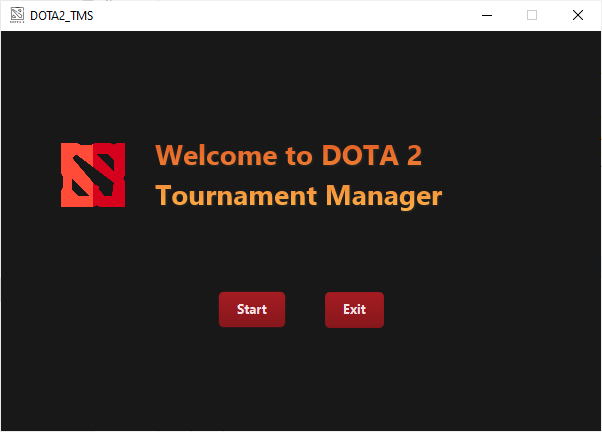
\includegraphics[width=0.5\textwidth]{figures/Welcome.png}
    \caption{Ekran powitalny \label{fig:welcome}}
\end{figure}

\section{Login.fxml}
Ekran logowania, gdzie można się zalogować lub zarejestrować lub wrócić do ekranu powitalnego.
\begin{figure}[H]
    \centering
    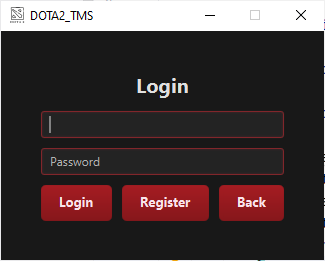
\includegraphics[width=0.5\textwidth]{figures/Login1.png}
    \caption{Ekran logowania \label{fig:login}}
\end{figure}
\begin{figure}[H]
    \centering
    \begin{subfigure}{0.7\linewidth}
        \centering
        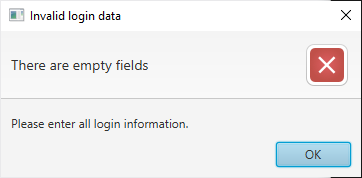
\includegraphics[width=.6\linewidth]{figures/FailedLogin1.png}
    \end{subfigure}
    \begin{subfigure}{0.7\linewidth}
        \centering
        \subcaption{\label{subfigure_a}}
        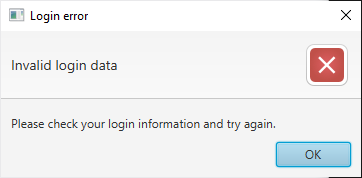
\includegraphics[width=.6\linewidth]{figures/FailedLoginData.png}
        \subcaption{\label{subfigure_b}}
    \end{subfigure}
    \begin{subfigure}{0.7\linewidth}
        \centering
        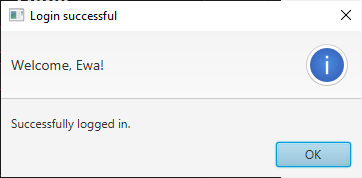
\includegraphics[width=.6\linewidth]{figures/SuccesLogin.png}
        \subcaption{\label{subfigure_c}}
    \end{subfigure}
    \caption{ Błedne i Udane logowania: \protect\subref{subfigure_a} Empty fields error, \protect\subref{subfigure_b} Invalid login data(nieznaleziono w db), \protect\subref{subfigure_c} Successful login. \label{fig:subcaption}}
\end{figure}
\section{Register.fxml}
Ekran rejestracji, gdzie można się zarejestrować lub wrócić do ekranu logowania. Przy logowaniu możesz wybrać rolę.
\begin{figure}[H]
    \centering
    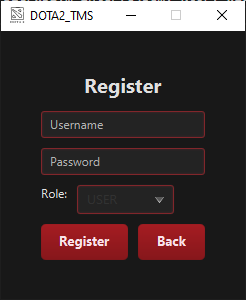
\includegraphics[width=0.4\textwidth]{figures/Register1.png}
    \caption{Ekran rejestracji z wybranym User \label{fig:register}}
\end{figure}
\begin{figure}[H]
    \centering
    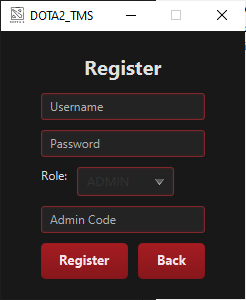
\includegraphics[width=0.4\textwidth]{figures/Register2.png}
    \caption{Ekran rejestracji z wybranym Admin \label{fig:register1}}
\end{figure}
\begin{figure}[H]
    \begin{subfigure}{0.5\textwidth}
        \centering
        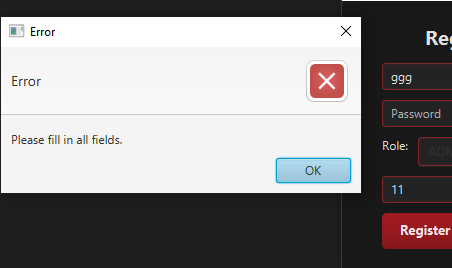
\includegraphics[width=.7\linewidth]{figures/ErrorFields.png}
        \subcaption{\label{subfigure_a}}
    \end{subfigure}
    \begin{subfigure}{0.5\textwidth}
        \centering
        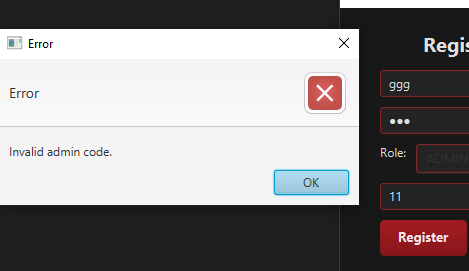
\includegraphics[width=.7\linewidth]{figures/ErrorCode.png}
        \subcaption{\label{subfigure_b}}
    \end{subfigure}
    \begin{subfigure}{0.5\textwidth}
        \centering
        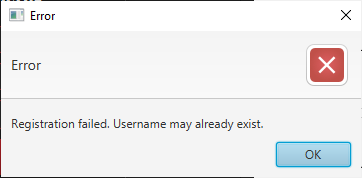
\includegraphics[width=.7\linewidth]{figures/ErrorExist.png}
        \subcaption{\label{subfigure_c}}
    \end{subfigure}
    \begin{subfigure}{0.5\textwidth}
        \centering
        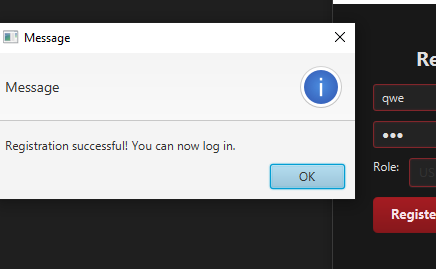
\includegraphics[width=.7\linewidth]{figures/SuccesRegister.png}
        \subcaption{\label{subfigure_d}}
    \end{subfigure}
    \caption{ Błedne i Udane rejestracji: \protect\subref{subfigure_a} Empty fields error, \protect\subref{subfigure_b} Invalid admin code, \protect\subref{subfigure_c} User already exists, \protect\subref{subfigure_d} Successful registration. \label{fig:subcaption}}
\end{figure}

\section{TournamentSelection.fxml}
Ekran wyboru turnieju, gdzie można wybrać dostępny turniej lub wylogować się i wrócić do ekranu logowania. Jeżeli jesteś adminem, możesz dodać, edytować lub usunąć turniej.\begin{figure}[H]
    \centering
    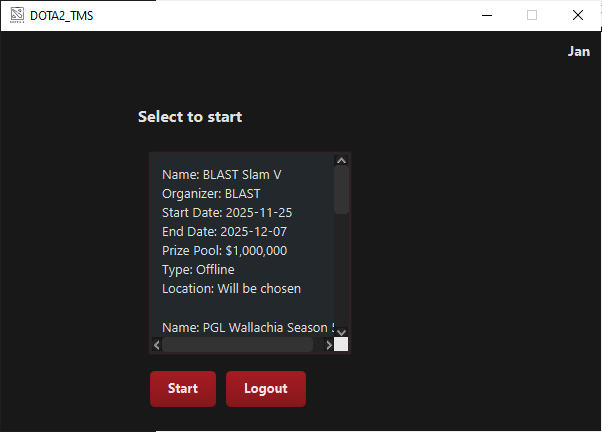
\includegraphics[width=0.4\textwidth]{figures/UserInterface.png}
    \caption{Ekran wyboru turnieju jako User \label{fig:tournament_selection}}
\end{figure}
\begin{figure}[H]
    \centering
    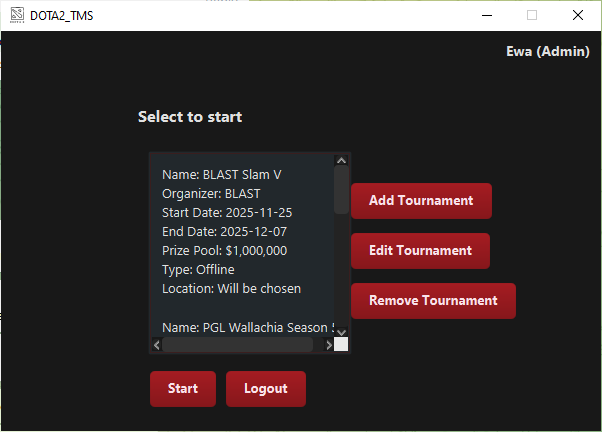
\includegraphics[width=0.4\textwidth]{figures/AdminInterface.png}
    \caption{Ekran wyboru turnieju jako Admin \label{fig:tournament_selection_admin}}
\end{figure}
\begin{figure}
    \centering
    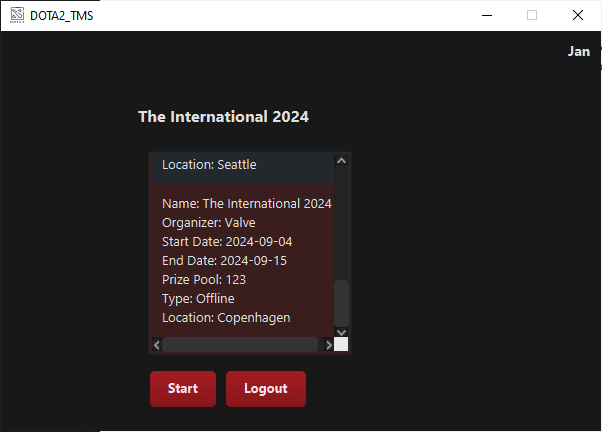
\includegraphics[width=0.4\textwidth]{figures/Chosen.png}
    \caption{Gdy klikasz na turniej górny label zmienia się \label{fig:tournament_selection_fxml}}
\end{figure}
\begin{figure}
    \centering
    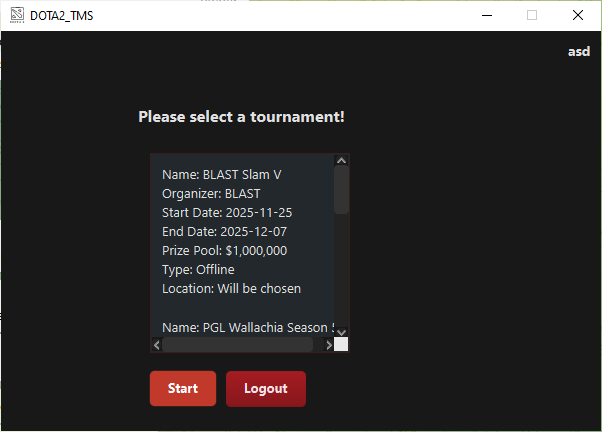
\includegraphics[width=0.4\textwidth]{figures/IfPressStart.png}
    \caption{Gdy klikasz start, prosi o wyborze turnieju \label{fig:tournament_selection_fxml_admin}}
\end{figure}
\begin{figure}[H]
    \centering
    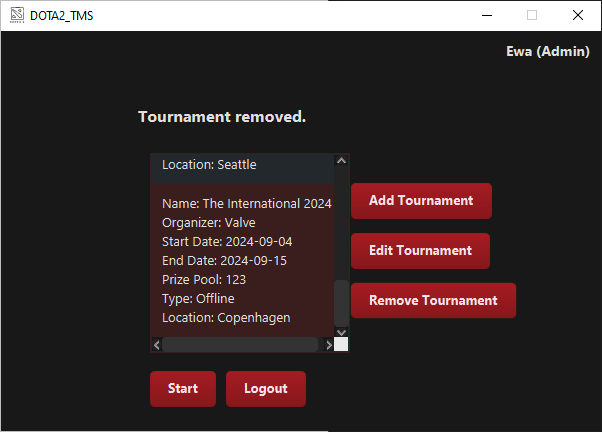
\includegraphics[width=0.4\textwidth]{figures/Removing.png}
    \caption{Gdy klikasz remove, wyrzuca go z bazy danych i tabeli, zmienia się górny label \label{fig:tournament_selection_fxml_remove}}
\end{figure}
\begin{figure}
    \centering
    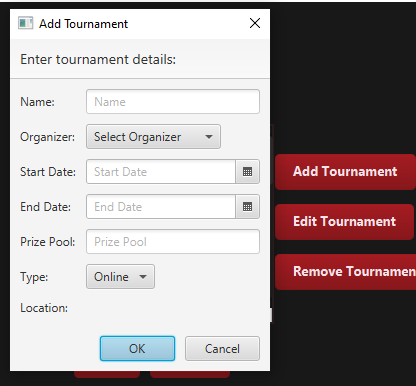
\includegraphics[width=0.4\textwidth]{figures/Add.png}
    \caption{Gdy klikasz add, otwiera się okno z formularzem do dodania turnieju \label{fig:tournament_selection_fxml_add}}
\end{figure}
\begin{figure}[H]
    \begin{subfigure}{0.3\textwidth}
        \centering
        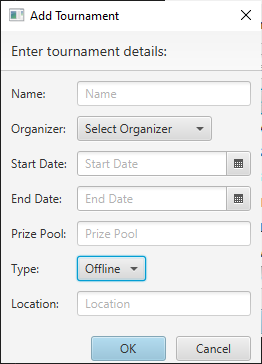
\includegraphics[width=.8\linewidth]{figures/AddOffline.png}
        \caption{Typ offline, pojawia sie miejsce prowadzenia \label{subfigure_name}}
    \end{subfigure}
    \begin{subfigure}{0.3\textwidth}
        \centering
        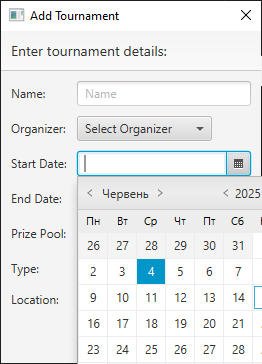
\includegraphics[width=.8\linewidth]{figures/SelectingData.png}
        \caption{Możesz wybrać dowolną datę rozpoczęcia turnieju \label{fig:tournament_selection_fxml_edit}}
    \end{subfigure}
    \begin{subfigure}{0.3\textwidth}
        \centering
        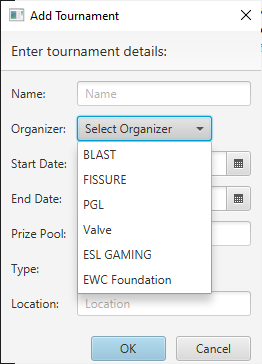
\includegraphics[width=.8\linewidth]{figures/SelectingOrganizer.png}
        \caption{Możesz wybrać organizatora turnieju \label{fig:tournament_selection_fxml_add_offline}}
    \end{subfigure}
    \caption{Formularz do dodania lub edycji turnieju: \protect\subref{subfigure_name}, \protect\subref{fig:tournament_selection_fxml_edit}, \protect\subref{fig:tournament_selection_fxml_add_offline}. \label{fig:tournament_selection_fxml_form}}
\end{figure}
\begin{figure}[H]
    \begin{subfigure}{0.6\textwidth}
        \centering
        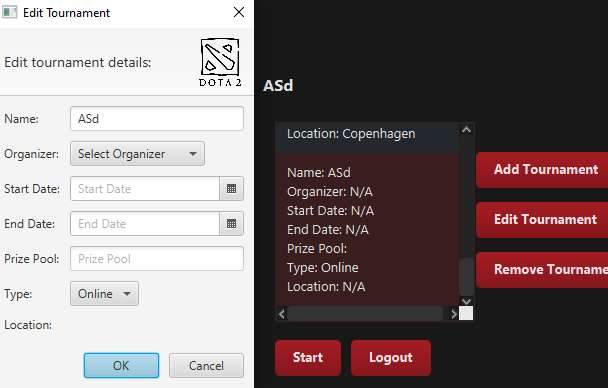
\includegraphics[width=.8\linewidth]{figures/Edit.png}
        \caption{Przy edycje już wprowadzone dane wypełniają odpowiene pola \label{subfigure_name}}
    \end{subfigure}
    \begin{subfigure}{0.6\textwidth}
        \centering
        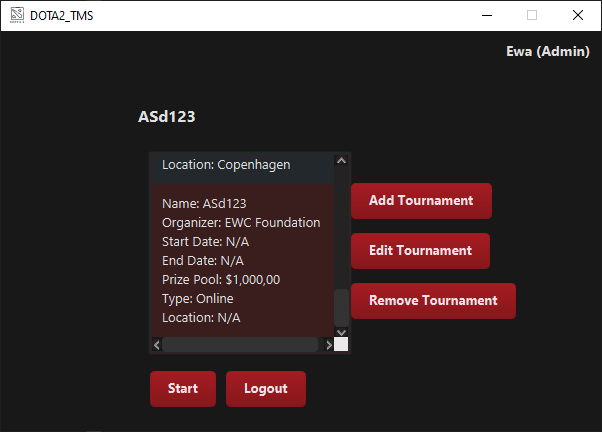
\includegraphics[width=.8\linewidth]{figures/Edited.png}
        \caption{Wprowadziłem jakieś zmiany w formularzu \label{fig:tournament_selection_fxml_edit}}
    \end{subfigure}
    \caption{Edycja turnieju: \protect\subref{subfigure_name}, \protect\subref{fig:tournament_selection_fxml_edit}. \label{fig:tournament_selection_fxml_edit_form}}
\end{figure}
\section{TournamentInfo.fxml}
Ekran informacji o turnieju, nie ma jeszcze żadnych odpowiednich funkcji, tylko Back żeby wrócić do wyboru.
\begin{figure}[H]
    \begin{subfigure}{0.6\textwidth}
        \centering
        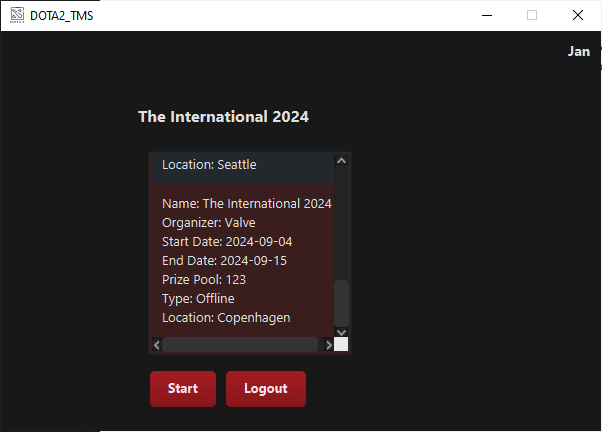
\includegraphics[width=.8\linewidth]{figures/Chosen.png}
        \caption{Wybieram jakiś turniej \label{subfigure_name}}
    \end{subfigure}
    \begin{subfigure}{0.6\textwidth}
        \centering
        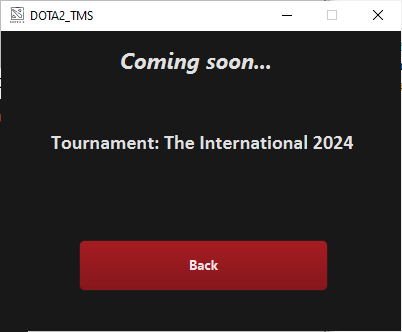
\includegraphics[width=.7\linewidth]{figures/Info.png}
        \caption{W przyszłości planowane są dodatkowe funkcje \label{fig:tournament_selection_fxml_edit}}
    \end{subfigure}
    \caption{Ekran informacji o turnieju: \protect\subref{subfigure_name}, \protect\subref{fig:tournament_selection_fxml_edit}. \label{fig:tournament_selection_fxml_edit_form}}
\end{figure}